\documentclass[12pt]{article}


\usepackage[utf8]{inputenc}
\usepackage[a4paper,top=3cm,bottom=2cm,left=3cm,right=3cm,marginparwidth=1.75cm]{geometry}
\usepackage[nodayofweek]{datetime}
\usepackage{tabularx}
\usepackage[small]{titlesec}
\usepackage{graphicx}
\usepackage{tabularx}
\usepackage{amsmath}
\usepackage{fancyvrb}
\newcolumntype{L}[1]{>{\raggedright\arraybackslash}p{#1}}
\newcolumntype{C}[1]{>{\centering\arraybackslash}p{#1}}
\newcolumntype{R}[1]{>{\raggedleft\arraybackslash}p{#1}}

\begin{document}

\begin{titlepage}
    \begin{center}
        \huge{\bfseries  Tribhuvan University}\\
        \Large{Institute of Engineering}\\
        \huge{ \bfseries  Pulchowk Campus}\\[3.2cm]


        \textsc{\Large Digital Signal Analysis and Processing}\\[-0.5cm]
        \line(1,0){400}\\
        \huge{\bfseries Lab 6}\\
        \large{IIR and FIR Filter Design}
        \line(1,0){400}\\


        \textsc{\Large Submitted by:}\\
        \Large Bishal Katuwal\\ \large 075BCT028\\    [0.85cm]

        \textsc{\Large Submitted to:}\\\
        \large Department of Electronics and Computer Engineering\\Pulchowk Campus\\    [0.85cm]
        
        \textsc{\Large Submitted on:}\\
        \today
        
    \end{center}
\end{titlepage}
\pagebreak
% ===============================================================
\paragraph{Title\\}
IIR and FIR Filter Design

\paragraph{Background Theory}
\subparagraph{Design of IIR Filters\\}
There are several methods that can be used to design digital filters having an infinite duration
unit sample response. One of the popular methods is based on converting an analog filter into a
digital filter. In this method we begin the design of digital filter in the analog domain and then
convert the design into the digital domain. For this purpose, depending on the specifications of
the required digital filter the various approximations like butterworth, chebyshev, chebyshev2
and elliptic filters are used. In this lab we deal with following approximations:
\begin{itemize}
    \item Butterworth Approximation
    \item Chebyshev Approximation
    \begin{itemize}
        \item Type I
        \item Type II
    \end{itemize}
    \item Elliptic Approximation
\end{itemize}
Among the different approaches used in the design of digital IIR filters this lab session deals
with the,
\begin{itemize}
    \item Impulse Invariance method\\
    In Impulse Invariance method, the objective is to design an IIR filter having an unit sample
response h(n) that is the sampled version of the impulse response of the analog filter.That is 
\begin{equation}
    \begin{aligned}
        h(n) = h(nT)&\\
        &n = 0,1,2,...\\
        &T \ is \ the \ sampling \ interval
    \end{aligned}
\end{equation}
    \item Bi-Linear Transformation\\
    In Bi-Linear transformation a conformal mapping from s plane to z plane is carried out with the
relation:
\begin{equation}
    s = \frac{2}{T}(\frac{1-z^{-1}}{1+z^{-1}})
\end{equation}
\end{itemize}

\subparagraph{Design of FIR Filters\\}
The major difficulty lies in the implementation of the non-iterative direct design method for IIR
filters. However FIR filters are almost entirely restricted to discrete-time implementations. Thus
the design techniques for FIR filters are based on directly approximating the desired frequency
response of the discrete time system. Furthermore, most techniques for approximating the
magnitude response of the FIR system assume a linear phase constraint; thereby avoiding the
problem of spectrum factorization that complicates the direct design of IIR filters.

The simplest method of FIR design is called the window method. This lab deals with following windows:
\begin{itemize}
    \item Rectangular window
    \item Bartlett window
    \item Blackmann window
    \item Hamming window
    \item Hanning window
    \item Kaiser window
\end{itemize}
\subparagraph{MATLAB\\}
{\bfseries Signal} package has following functions for filter design.\\
{\large For IIR}
\begin{itemize}
    \item {\bfseries besselap} : Return bessel analog filter prototype.
    \item {\bfseries besself} : Generate a Bessel filter.
    \item {\bfseries bilinear} : Transform a s-plane filter specification into a z-plane specification.
    \item {\bfseries buttap} : Design lowpass analog Butterworth filter.
    \item {\bfseries butter} : Generate a Butterworth filter.
    \item {\bfseries buttord} : Compute the minimum filter order of a Butterworth filter with the desired response characteristics.
    \item {\bfseries cheb} : Returns the value of the nth-order Chebyshev polynomial calculated at the point x.
    \item {\bfseries cheb1ap} : Design lowpass analog Chebyshev type I filter.
    \item {\bfseries cheb1ord} : Compute the minimum filter order of a Chebyshev type I filter with the desired response characteristics.
    \item {\bfseries cheb2ap} : Design lowpass analog Chebyshev type II filter.
    \item {\bfseries cheb2ord} : Compute the minimum filter order of a Chebyshev type II filter with the desired response characteristics.
    \item {\bfseries cheby1} : Generate a Chebyshev type I filter with RP dB of passband ripple.
    \item {\bfseries cheby2} : Generate a Chebyshev type II filter with RS dB of stopband attenuation.
    \item {\bfseries ellip} : Generate an elliptic or Cauer filter with RP dB of passband ripple and RS dB of stopband attenuation.
    \item {\bfseries ellipap} : Design lowpass analog elliptic filter.
    \item {\bfseries ellipord} : Compute the minimum filter order of an elliptic filter with the desired response characteristics.
    \item {\bfseries iirlp2mb} : IIR Low Pass Filter to Multiband Filter Transformation
    \item {\bfseries impinvar} : Converts analog filter with coefficients B and A to digital, conserving impulse response.
    \item {\bfseries invimpinvar} : Converts digital filter with coefficients B and A to analog, conserving impulse response.
    \item {\bfseries ncauer} : Analog prototype for Cauer filter.
    \item {\bfseries pei\_tseng\_notch} : Return coefficients for an IIR notch-filter with one or more filter frequencies and according (very narrow) bandwidths to be used with 'filter' or 'filtfilt'.
    \item {\bfseries sftrans} : Transform band edges of a generic lowpass filter (cutoff at W=1) represented in splane zero-pole-gain form.

    {\large For FIR}
    \item {\bfseries barthannwin} :   Return the filter coefficients of a modified Bartlett-Hann window of length M.
    \item {\bfseries blackmanharris} : Return the filter coefficients of a Blackman-Harris window of length M.
    \item {\bfseries blackmannuttall} : Return the filter coefficients of a Blackman-Nuttall window of length M.
    \item {\bfseries boxcar} : Return the filter coefficients of a rectangular window of length M.
    \item {\bfseries chebwin} : Return the filter coefficients of a Dolph-Chebyshev window of length M.
    \item {\bfseries hann} : Return the filter coefficients of a Hanning window of length M.
    \item {\bfseries kaiser} :  Return the filter coefficients of a Kaiser window of length M.
    \item {\bfseries rectwin} : Return the filter coefficients of a rectangular window of length M.
    \item {\bfseries triang} : Return the filter coefficients of a triangular window of length M.
    \item {\bfseries window} : Create an M-point window from the function F.
\end{itemize}
% ==========================================
\pagebreak
\paragraph{Activity}
\begin{enumerate}
    \item Butterworth approximation
    \begin{Verbatim}[frame = single]
pkg load signal
wp=0.2*pi;
ws=0.5*pi;
As=30;
Ap=0.4;
[N,wn]=buttord(wp/pi,ws/pi,Ap,As);
[b,a]=butter(N,wn);
freqz(b,a);
    \end{Verbatim}
    \begin{figure}[h!]
        \centering
        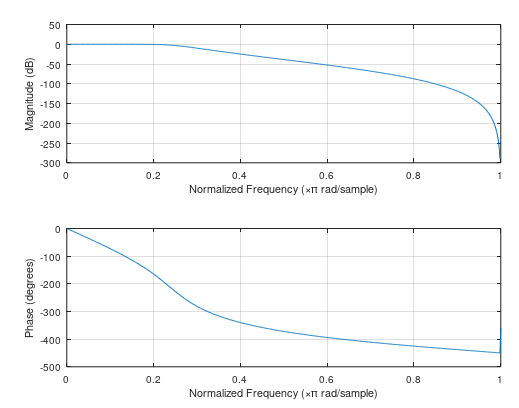
\includegraphics{labss/Lab6_1.PNG}
        \caption{Butterworth approximation}
    \end{figure}
    \item For data sampled at 1000 Hz, design a lowpass filter with less than 3 dB of ripple in the
    passband defined from 0 to 40 Hz and at least 60 dB of ripple in the stopband defined from 
    150 Hz to the Nyquist frequency (500 Hz):
    \begin{itemize}
        \item Chebyshev I
        \begin{Verbatim}[frame = single]
pkg load signal

Wp = 40/500;
Ws = 150/500;
Rp = 3;
Rs = 60;

[n,Wn] = cheb1ord(Wp,Ws,Rp,Rs);
[b,a] = cheby1(n,Rp,Wn);
freqz(b,a,512,1000);
title('Chebyshev Type I Lowpass Filter')
                \end{Verbatim}
                \begin{figure}[h!]
                    \centering
                    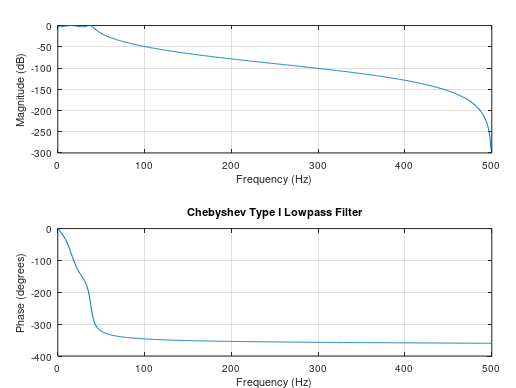
\includegraphics{labss/Lab6_2a.PNG}
                    \caption{Chebyshev I approximation}
                \end{figure}
        \item Chebyshev II
    \end{itemize}
    \begin{Verbatim}[frame = single]
pkg load signal

Wp = 40/500;
Ws = 150/500;
Rp = 3;
Rs = 60;

[n,Wn] = cheb2ord(Wp,Ws,Rp,Rs);
[b,a] = cheby2(n,Rp,Wn);
freqz(b,a,512,1000);
title('Chebyshev Type II Lowpass Filter')
            \end{Verbatim}
            \begin{figure}[h!]
                \centering
                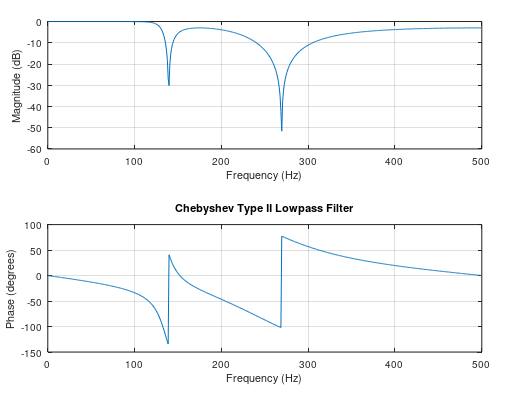
\includegraphics{labss/Lab6_2b.PNG}
                \caption{Chebyshev II approximation}
            \end{figure}
            \pagebreak
\item Design a bandpass filter with a passband of 60 Hz to 200 Hz, with less than 3 dB of ripple in
the passband, and 40 dB attenuation in the stopbands that are 50 Hz wide on both sides of the
passband:
\begin{itemize}
    
    \item Chebyshev I
    \begin{Verbatim}[frame = single]
pkg load signal

Wp = [60 200]/500;
Ws = [50 250]/500;
Rp = 3; Rs = 40;
[n,Wn] = cheb1ord(Wp,Ws,Rp,Rs);
[b,a] = cheby1(n,Rp,Wn);
freqz(b,a,512,1000);
title('Chebyshev Type I Bandpass Filter')
                    \end{Verbatim}
                    \begin{figure}[h!]
                        \centering
                        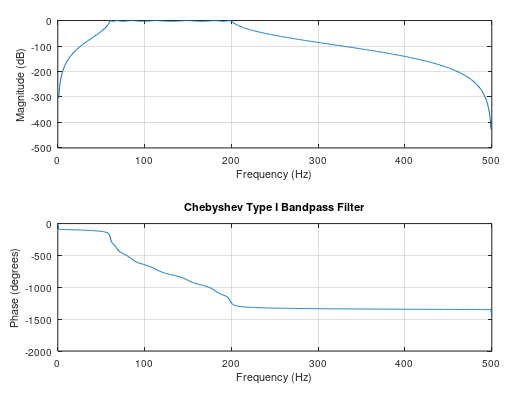
\includegraphics{labss/Lab6_3a.PNG}
                        \caption{Chebyshev I approximation}
                    \end{figure}
                    \pagebreak
    \item Chebyshev II
    \begin{Verbatim}[frame = single]
pkg load signal

Wp = [60 200]/500;
Ws = [50 250]/500;
Rp = 3; Rs = 40;
[n,Wn] = cheb2ord(Wp,Ws,Rp,Rs);
[b,a] = cheby2(n,Rp,Wn);
freqz(b,a,512,1000);
title('Chebyshev Type II Bandpass Filter')
                            \end{Verbatim}
                            \begin{figure}[h!]
                                \centering
                                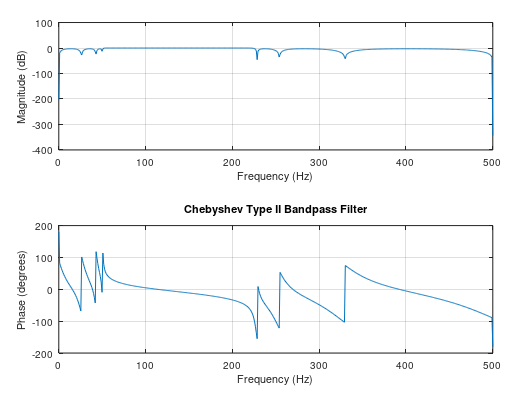
\includegraphics{labss/Lab6_3b.PNG}
                                \caption{Chebyshev II approximation}
                            \end{figure}
                            \pagebreak
\end{itemize}

\item Comparison of Butterworth, Chebyshev (I and II) and Elliptical approximations:
\begin{Verbatim}[frame = single]
pkg load signal

fc = 3e6; %cut-off frequency
fs = 10e6; %sampling frquency
n = 6; %order of the filter
As = 40; %Stopband attenuation in dB
Rp = 5; %Passband ripple in dB
[b,a] = butter(n,fc/(fs/2)); 
[h_butter,w_butter] = freqz(b,a,512);
[b,a] = cheby1(n,Rp,fc/(fs/2));
[h_cheby1,w_cheby1] = freqz(b,a,512);
[b,a] = cheby2(n,As,fc/(fs/2));
[h_cheby2,w_cheby2] = freqz(b,a,512);
[b,a] = ellip(n,Rp,As,fc/(fs/2));
[h_ellip,w_ellip] = freqz(b,a,512);
figure;
plot(w_butter/pi,20*log10(abs(h_butter)),'lineWidth',1.2); 
hold on
plot(w_cheby1/pi,20*log10(abs(h_cheby1)),'lineWidth',1.2); 
hold on
plot(w_cheby2/pi,20*log10(abs(h_cheby2)),'lineWidth',1.2); 
hold on
plot(w_ellip/pi,20*log10(abs(h_ellip)),'lineWidth',1.2)
ylim([-100 10]);grid on;
xlabel('Normalized Frequency (\times\pi rad/sample)')
ylabel('Magnitude (dB)')
legend('Butterworth','Cheby1','Cheby2','Elliptic','FontSize',10)
figure;
plot(w_butter/pi,unwrap(angle(h_butter)),'lineWidth',1.2); 
hold on
plot(w_cheby1/pi,unwrap(angle(h_cheby1)),'lineWidth',1.2); 
hold on
plot(w_cheby2/pi,unwrap(angle(h_cheby2)),'lineWidth',1.2); 
hold on
plot(w_ellip/pi,unwrap(angle(h_ellip)),'lineWidth',1.2); 
hold on
grid on;
xlabel('Normalized Frequency (\times\pi rad/sample)')
ylabel('Phase (radians)')
legend('Butterworth','Cheby1','Cheby2','Elliptic','FontSize',10)
                                \end{Verbatim}
                                \begin{figure}[h!]
                                    \centering
                                    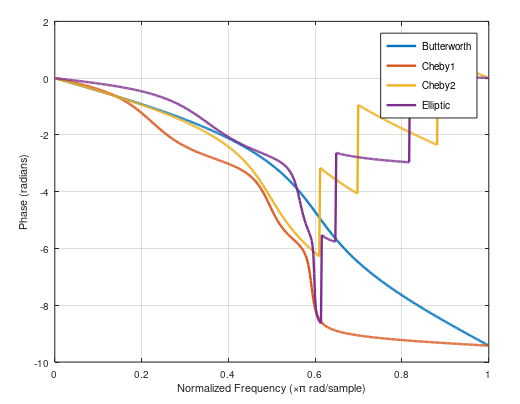
\includegraphics{labss/Lab6_4a.PNG}
                                    \caption{Phase comparisonn}

                                    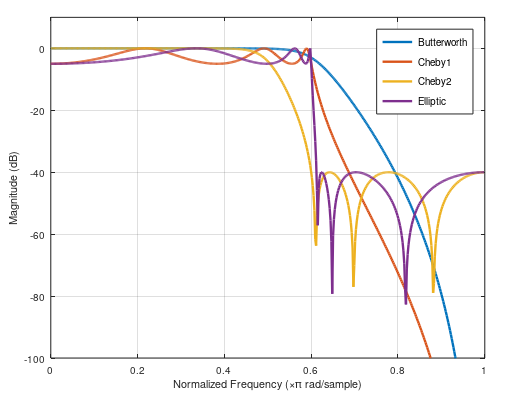
\includegraphics{labss/Lab6_4b.PNG}
                                    \caption{Magnitude comparison}
                                \end{figure}
                                \pagebreak
\item FIR filters
\begin{enumerate}
    \item Rectangular window
    \begin{Verbatim}[frame = single]
N=6;
wc=0.4*pi;
h=fir1(N,wc/pi,rectwin(N+1));
freqz(h);
    \end{Verbatim}
    \begin{figure}[h!]
        \centering
        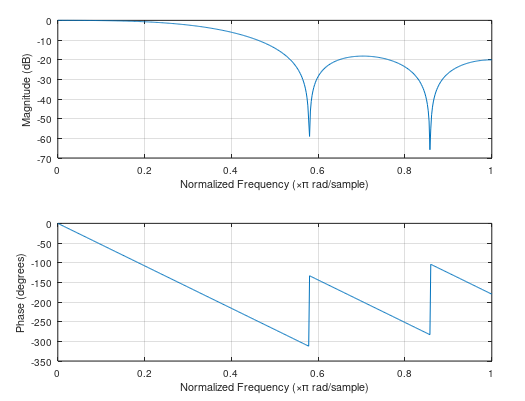
\includegraphics{labss/Lab6_5a.PNG}
        \caption{Rectangular window}
    \end{figure}
    \item Hanning window
    \begin{Verbatim}[frame = single]
N=6;
wc=0.4*pi;
h=fir1(N,wc/pi,hanning(N+1));
freqz(h);
    \end{Verbatim}
    \begin{figure}[h!]
        \centering
        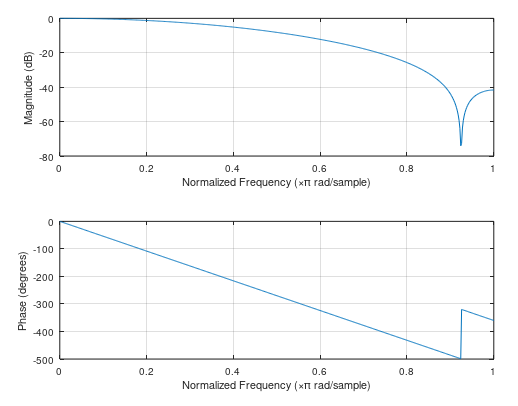
\includegraphics{labss/Lab6_5b.PNG}
        \caption{Hanning window}
    \end{figure}
    \pagebreak
    \item Hamming window
    \begin{Verbatim}[frame = single]
N=6;
wc=0.4*pi;
h=fir1(N,wc/pi,hamming(N+1));
freqz(h);
    \end{Verbatim}
    \begin{figure}[h!]
        \centering
        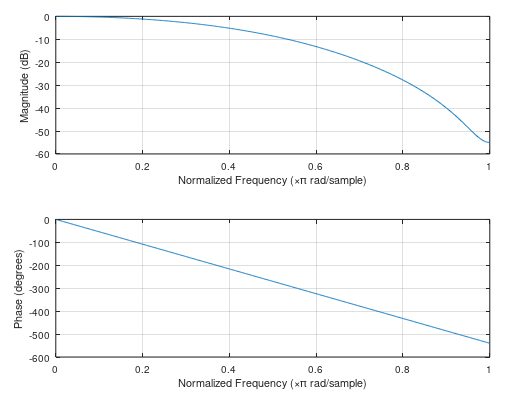
\includegraphics{labss/Lab6_5c.PNG}
        \caption{Hamming window}
    \end{figure}
    \pagebreak
    \item Bartlett window
    \begin{Verbatim}[frame = single]
N=6;
wc=0.4*pi;
h=fir1(N,wc/pi,bartlett(N+1));
freqz(h);
    \end{Verbatim}
    \begin{figure}[h!]
        \centering
        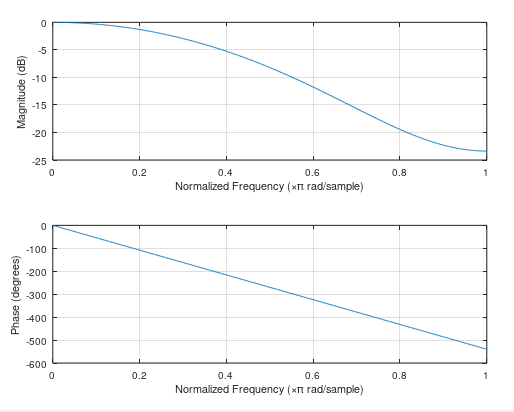
\includegraphics{labss/Lab6_5d.PNG}
        \caption{Bartlett window}
    \end{figure}
    \pagebreak
    \item Blackman window
    \begin{Verbatim}[frame = single]
N=6;
wc=0.4*pi;
h=fir1(N,wc/pi,blackman(N+1));
freqz(h);
    \end{Verbatim}
    \begin{figure}[h!]
        \centering
        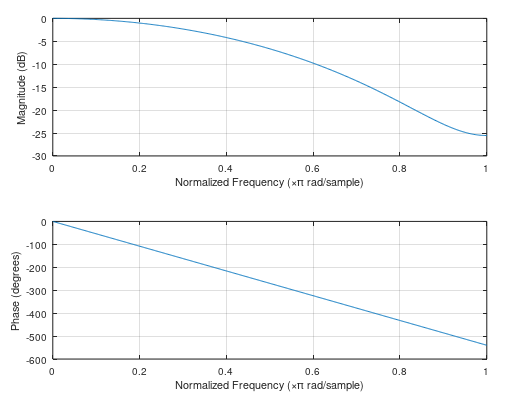
\includegraphics{labss/Lab6_5e.PNG}
        \caption{Blackman window}
    \end{figure}
    \pagebreak
    \item Kaiser window
    \begin{Verbatim}[frame = single]
N=6;
wc=0.4*pi;
h=fir1(N,wc/pi,kaiser(N+1));
freqz(h);
    \end{Verbatim}
    \begin{figure}[h!]
        \centering
        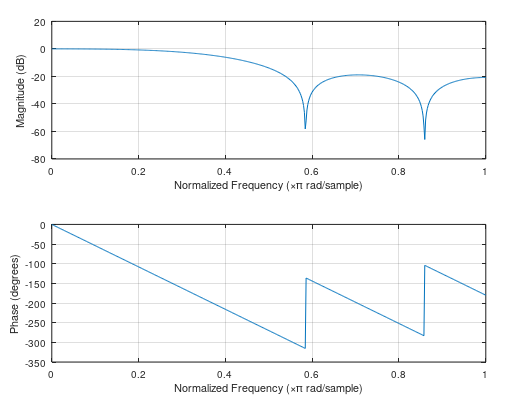
\includegraphics{labss/Lab6_5f.PNG}
        \caption{Kaiser window}
    \end{figure}
    \pagebreak
\end{enumerate}
\end{enumerate}
\paragraph{Conclusion\\}
In this way, "Lab 6 : IIR and FIR Filter Design" was completed with the help of MATLAB.
FIR filter was designed using Butterworth, Chebyshev approximation, and IIR filter was
designed using windowing method. Different windows like Blackman, Hanning, Hamming,
Rectangular, and Bartlett windows were used to design the FIR filter.
\end{document}